\documentclass[a4paper]{extarticle}
\usepackage[utf8]{inputenc}
\usepackage[a4paper, margin=1in]{geometry}

\usepackage{amssymb}
\usepackage{amsmath}
\usepackage{enumitem}
\usepackage{tcolorbox}
\usepackage{fancyhdr}
\usepackage{graphicx}
\usepackage{float}

\setlength{\parindent}{0em}
\setlength{\parskip}{0.4em}

\definecolor{theoremblue}{RGB}{1, 73, 124}
\definecolor{corollaryblue}{RGB}{70, 143, 175}
\definecolor{exampleblue}{RGB}{137, 194, 217}

\newtcolorbox{tbox}{colback=theoremblue!20,colframe=theoremblue,
boxrule=0pt,arc=0pt,boxsep=2pt,left=2pt,right=2pt,leftrule=2pt}

\newtcolorbox{cbox}{colback=corollaryblue!20,colframe=corollaryblue,
boxrule=0pt,arc=0pt,boxsep=2pt,left=2pt,right=2pt,leftrule=2pt}

\newtcolorbox{ebox}{colback=exampleblue!20,colframe=exampleblue,
boxrule=0pt,arc=0pt,boxsep=2pt,left=2pt,right=2pt,leftrule=2pt}

\title{IntroML - Lecture Notes Week 8}
\author{Ruben Schenk, ruben.schenk@inf.ethz.ch}
\date{\today}

\pagestyle{fancy}
\fancyhf{}
\rhead{ruben.schenk@inf.ethz.ch}
\rfoot{Page \thepage}
\lhead{IntroML - Lecture Notes Week 8}

\begin{document}

\maketitle

\section{PyTorch Tutorial}

\textbf{Autodiff} is an automatic implementation in PyTorch which calculates the gradients automatically given the \textit{forward pass} (i.e. the chain of operations from input to output).

\begin{figure}[H]
    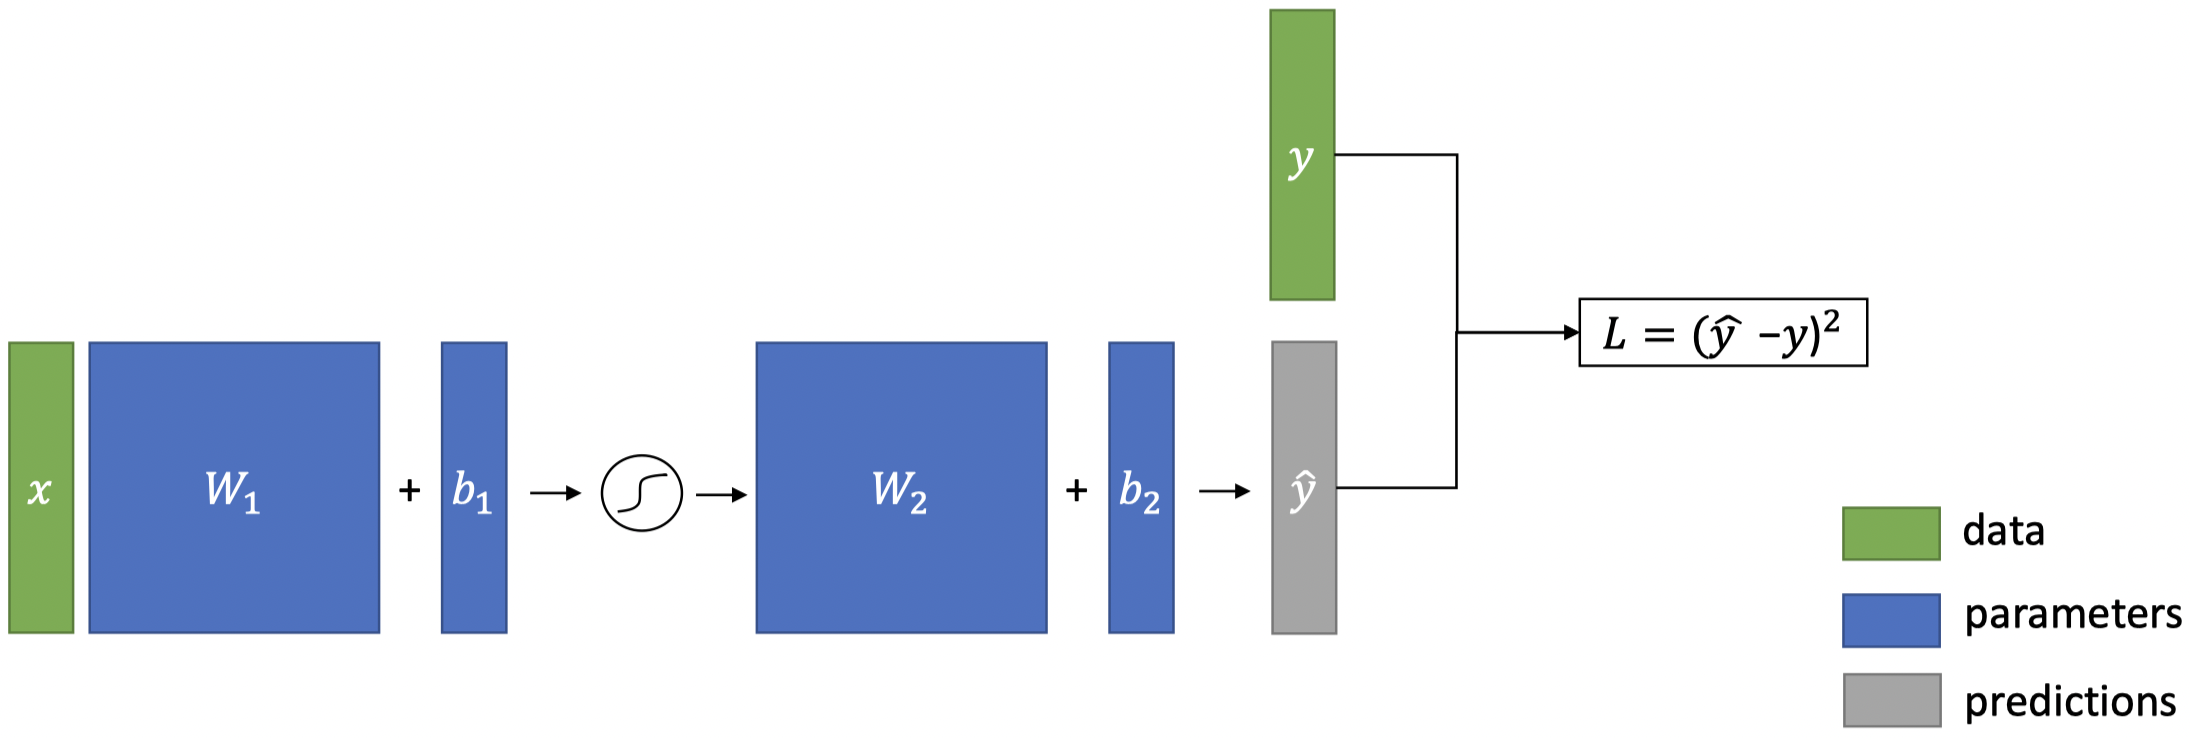
\includegraphics[width=15cm]{../images/IntroML_Fig8-1}
    \centering
\end{figure}

Given this forward pass, PyTorch automatically computes the derivatives (\textit{backward pass}) for us!

How does Autodiff work? First, as already mentioned, we need to provide the forward pass. Given that, PyTorch constructs the computation graph (DAG) and stores the intermediate computed values at each node of the graph.

Example: Consider the following simple function:
\begin{verbatim}
    def f(x, y):
        c = x + y
        d = c**2
        return x * d

    x = torch.tensor([3.0], requires_grad=True)
    y = torch.tensor([-1.0], requires_grad=True)
    f_val = f(x, y)
\end{verbatim}

For this function, we get the following forward pass:

\begin{figure}[H]
    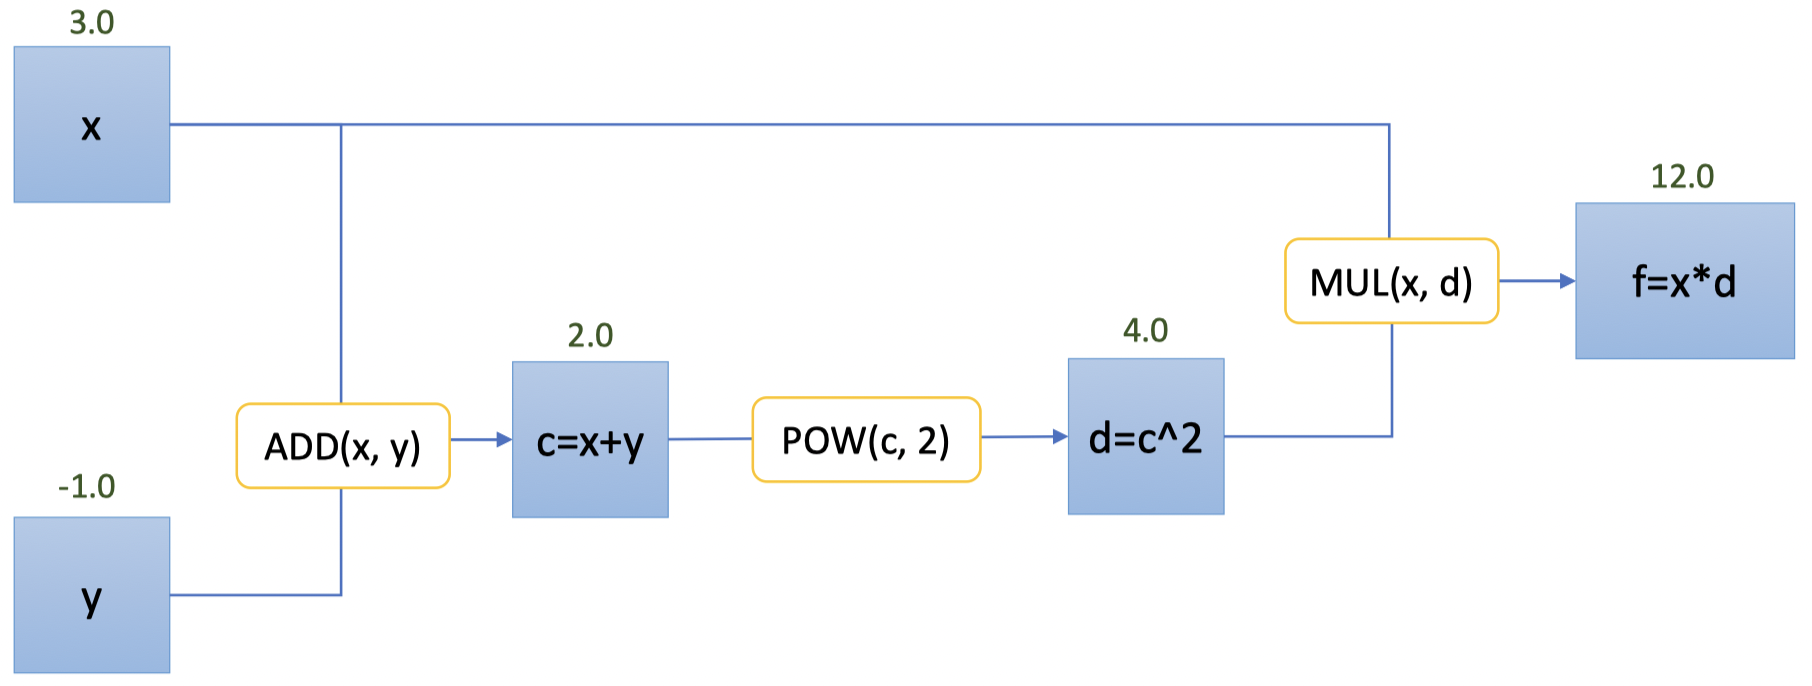
\includegraphics[width=15cm]{../images/IntroML_Fig8-2}
    \centering
\end{figure}

It is important to note here that every intermediate result is itself a tensor. Even if we override a variable, the previous tensor is kept alive.

Finally, Autodiff calculates the backward pass the following way:
\begin{itemize}
    \item Go back from the root (i.e. the loss) to the leaves (i.e. the parameters)
    \item Each elementary operation has a "backward function" that computes its derivatives
    \item We apply the chain rule along each path
    \item Total derivative is the sum of all path derivatives from the root to the leaf
\end{itemize}

\begin{figure}[H]
    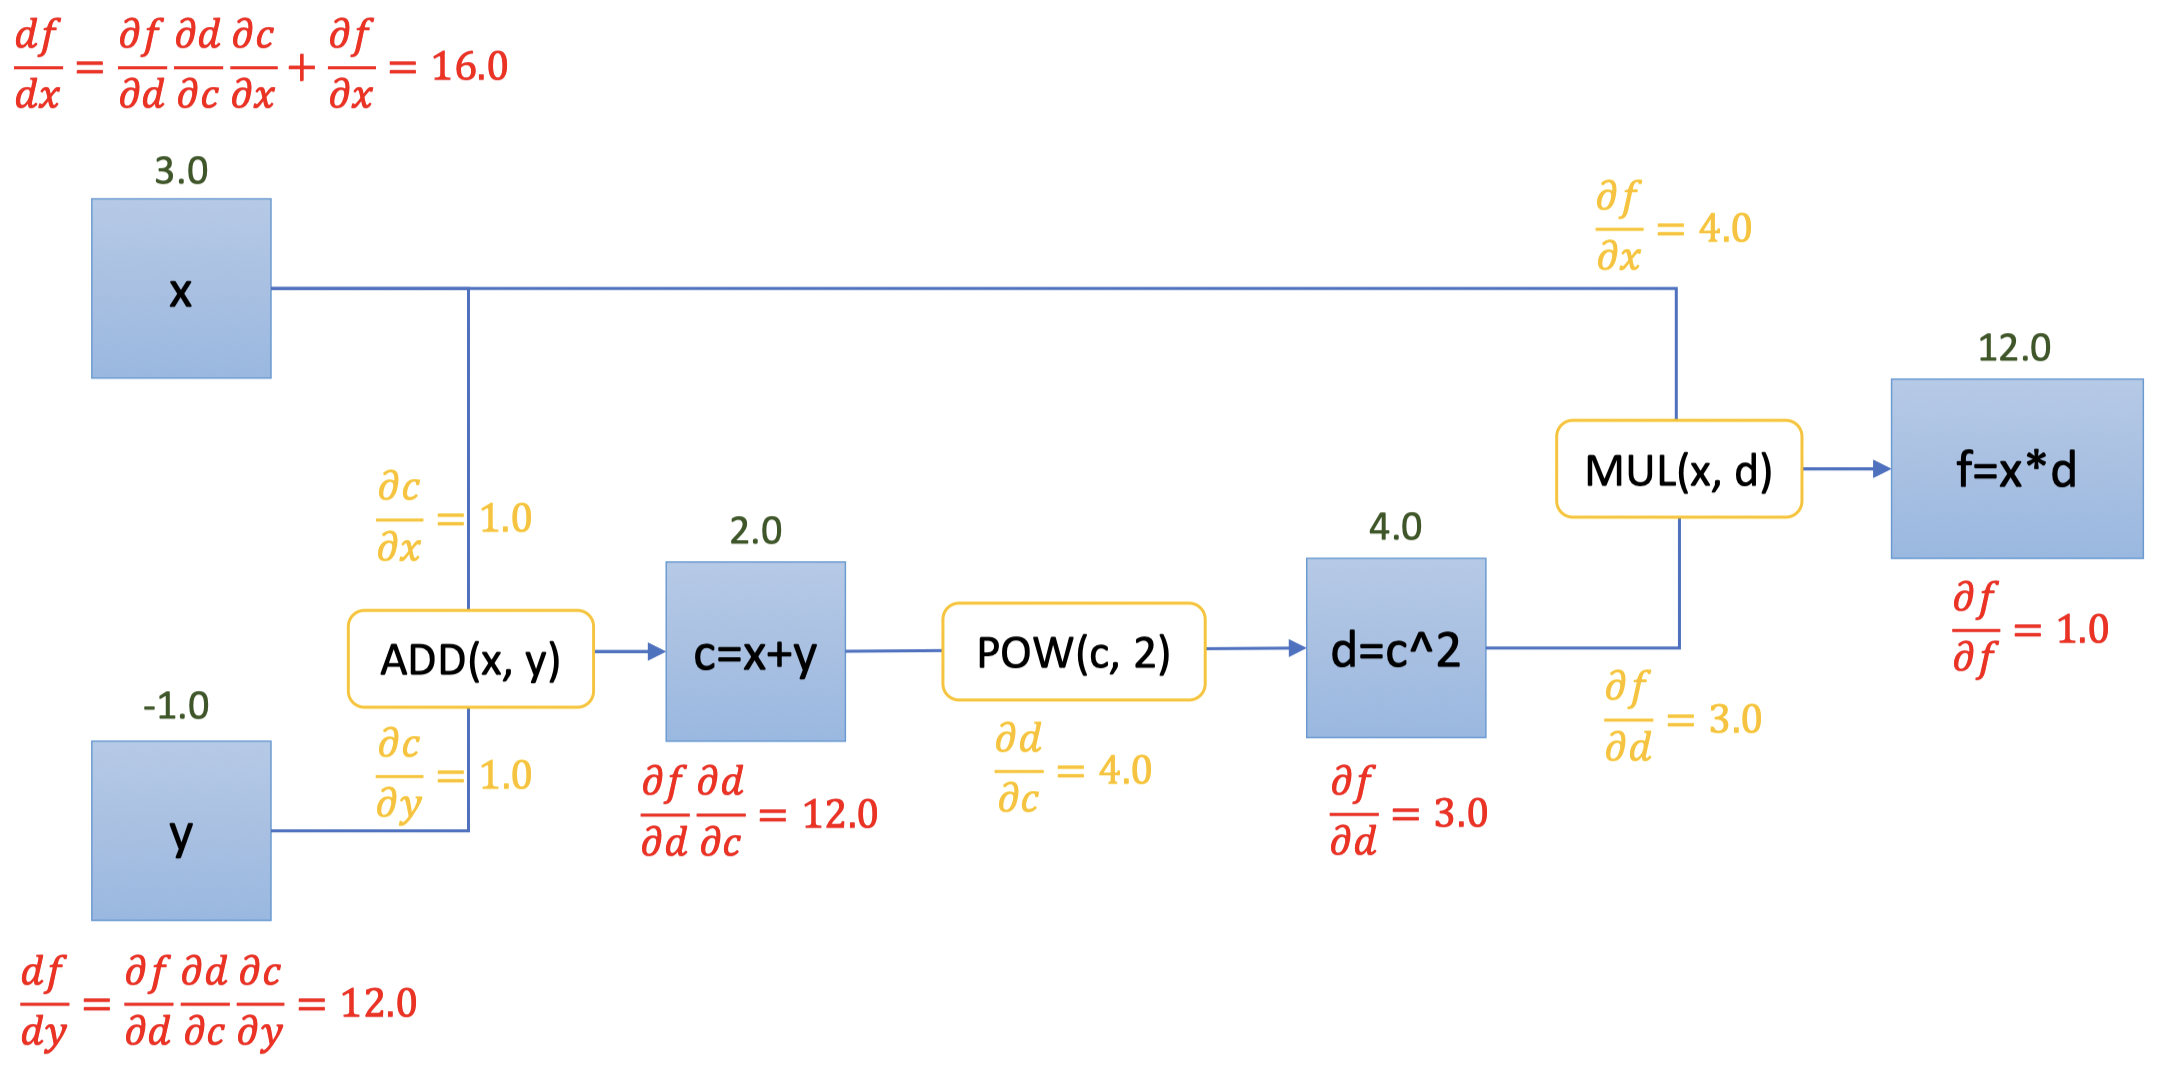
\includegraphics[width=15cm]{../images/IntroML_Fig8-3}
    \centering
\end{figure}

\section{Unsupervised Learning: Clustering}



\end{document}